%%%%%%%%%%%%%%%%%%%%%%%%%%%%%%%%%%%%%%%%%
% Stylish Article
% LaTeX Template
% Version 2.2 (2020-10-22)
%
% This template has been downloaded from:
% http://www.LaTeXTemplates.com
% https://www.latextemplates.com/template/stylish-article
%
% Original author:
% Mathias Legrand (legrand.mathias@gmail.com) 
% With extensive modifications by:
% Vel (vel@latextemplates.com)
%
% License:
% CC BY-NC-SA 3.0 (http://creativecommons.org/licenses/by-nc-sa/3.0/)
%
%%%%%%%%%%%%%%%%%%%%%%%%%%%%%%%%%%%%%%%%%

%----------------------------------------------------------------------------------------
%	PACKAGES AND OTHER DOCUMENT CONFIGURATIONS
%----------------------------------------------------------------------------------------

\documentclass[fleqn,10pt]{SelfArx} % Document font size and equations flushed left

\usepackage[english]{babel} % Specify a different language here - english by default

\usepackage{lipsum} % Required to insert dummy text. To be removed otherwise

\usepackage{epigraph}

\usepackage{tabularx}
\usepackage{booktabs}
\usepackage{multirow}
\usepackage[table,xcdraw]{xcolor}
\usepackage{adjustbox}
\usepackage{tablefootnote}
\newcolumntype{C}[1]{>{\centering\let\newline\\\arraybackslash\hspace{0pt}}m{#1}}

\usepackage{./msc}

%----------------------------------------------------------------------------------------
%	COLUMNS
%----------------------------------------------------------------------------------------

\setlength{\columnsep}{0.55cm} % Distance between the two columns of text
\setlength{\fboxrule}{0.75pt} % Width of the border around the abstract

%----------------------------------------------------------------------------------------
%	COLORS
%----------------------------------------------------------------------------------------

\definecolor{color1}{RGB}{0,0,90} % Color of the article title and sections
\definecolor{color2}{RGB}{0,20,20} % Color of the boxes behind the abstract and headings
\definecolor{keys1}{rgb}{0.0, 0.29, 0.33}
\definecolor{keys2}{rgb}{0.25, 0.7, 0.55}
\definecolor{keys3}{rgb}{0.1, 0.3, 0.4}
\definecolor{keys4}{rgb}{0.21, 0.46, 0.53}
\definecolor{strings}{rgb}{0.0, 0.47, 0.44}
\definecolor{comments}{rgb}{0.4, 0.4, 0.5}
\definecolor{terminaltext}{rgb}{1,1,1}
\definecolor{terminalbackground}{rgb}{0.2,0.2,0.3}

%----------------------------------------------------------------------------------------
%	BLOCKS
%----------------------------------------------------------------------------------------

\usepackage[framemethod=TikZ]{mdframed}
\newcounter{definition}[section]\setcounter{definition}{0}
\newcommand{\thedef}{\arabic{section}.\arabic{definition}}
\newenvironment{definition}[2][]{%
    \refstepcounter{definition}
 
    % Code for box design goes here.
	\ifstrempty{#1}%
	% if condition (without title)
	{\mdfsetup{%
	    frametitle={%
	        \tikz[baseline=(current bounding box.east),outer sep=0pt]
	        \node[anchor=east,rectangle,fill=color2!10]
	        {\strut Definition~\thedef};}
	    }%
	% else condition (with title)
	}{\mdfsetup{%
	    frametitle={%
	        \tikz[baseline=(current bounding box.east),outer sep=0pt]
	        \node[anchor=east,rectangle,fill=color2!10]
	        {\strut Definition~\thedef:~#1};}%
	    }%
	}%
	% Both conditions
	\mdfsetup{%
	    innertopmargin=10pt,linecolor=color2!10,%
	    linewidth=1pt,topline=true,%
	    frametitleaboveskip=\dimexpr-\ht\strutbox\relax%
	}
 
\begin{mdframed}[]\relax}{%
\end{mdframed}}

%----------------------------------------------------------------------------------------
%	HYPERLINKS
%----------------------------------------------------------------------------------------

\usepackage{hyperref} % Required for hyperlinks

\hypersetup{
	hidelinks,
	colorlinks,
	breaklinks=true,
	urlcolor=color2,
	citecolor=color1,
	linkcolor=color1,
	bookmarksopen=false,
	pdftitle={Title},
	pdfauthor={Author},
}

%----------------------------------------------------------------------------------------
%	ARTICLE INFORMATION
%----------------------------------------------------------------------------------------

\Subject{Computer Network Security seminar} % Journal information
\AcademicYear{A.Y. 2022/2023} % Additional notes (e.g. copyright, DOI, review/research article)

\PaperTitle{Automated Symbolic Verification of the Needham-Schroeder Protocol} % Article title

\Authors{Denis D'Ambrosi\textsuperscript{1}} % Authors
\affiliation{\textsuperscript{1}\textit{Student number 147681}, \lstinline|dambrosi.denis@spes.uniud.it|} % Author affiliation

\Keywords{Network Security --- Automated Verification --- Formal Verification} % Keywords - if you don't want any simply remove all the text between the curly brackets
\newcommand{\keywordname}{Keywords} % Defines the keywords heading name

%----------------------------------------------------------------------------------------
%	ABSTRACT
%----------------------------------------------------------------------------------------

\Abstract{As cryptographic protocols become both more complicated and more critical by the day, we must find a way to systematically verify message exchanges without the added burden of manual proving. To solve this issue, multiple theorem provers have been proposed in the last years, each one with its flaws and advantages. In this paper, we deal with the Tamarin prover, an automated tool that exploits multiset rewriting rules and guarded fragments of temporal logic to model cryptographic protocols and check their security properties. After an initial introduction to the topic as a whole, we dig deeper into the tool from a user's perspective and show how a simple key exchange protocol (the symmetric Needham-Schroeder protocol) can be modeled within a logic theory. This example will allows us to show how easily some message exchanges can be formalized within this prover; on the other hand, it will also demonstrate how the unbounded nature of this tools will require us to take some further assumptions on the protocol in order to avoid non-termination.}

%----------------------------------------------------------------------------------------
\renewcommand*{\ttdefault}{qcr}
\begin{document}

\maketitle % Output the title and abstract box

\tableofcontents % Output the contents section

\thispagestyle{empty} % Removes page numbering from the first page

%----------------------------------------------------------------------------------------
%	ARTICLE CONTENTS
%----------------------------------------------------------------------------------------

\section*{Introduction} % The \section*{} command stops section numbering

\addcontentsline{toc}{section}{Introduction} % Adds this section to the table of contents

\epigraph{Security protocols are three-line programs that people still manage to get wrong}{Roger M. Needham}

As computing becomes more obiquitous and distributed, we need an ever-increasing amount of cryptographic protocols to allow different parties to share information in a confidential, authenticated and integral way. New communication protocols are being deployed by the day, but most of them have at least some hidden flaw that, once found, can compromise the security of the communication, with potentially catastrophic effects. To avoid such a disaster, our best defense is to actually verify said protocols in some formal model, that will ensure us that, at least within the assumptions of the model itself, the exchange can not be exploited maliciously. Writing these proof by hand is often a cumbersome, long and error-prone process, thus in the last years computer scientists and mathematicians have instead started relying on automated tools that can carry on the demonstration for them. In this essay, we will take a closer look at one of such tools (the Tamarin prover \cite{tamarin}), by presenting its syntax, strengths, limitations and a practical example of modelization.

The essay is structured as follows: in section \ref{sec:SymbolicModel} we will briefly introduce one of such formal verification models, in section \ref{sec:TamarinOverview} we will give an introduction to the Tamarin prover from a user's perspective, while in the following section we will show how such tool can be used for real-world formal verification by modeling the Needham-Schroeder Symmetric protocol. Finally, in section \ref{sec:conclusions} we will summarize the results of this paper.

\section{The Dolev Yao model}\label{sec:SymbolicModel}

When dealing with the verification of internet protocols, two (main) paradigms are used to formally prove the security properties of both new and established message exchanges: the computational and the symbolic models. The first, initially introduced by Goldwasser, Micali \cite{goldwasser}, Rivest \cite{rivest}, Yao \cite{yao} and others, treats messages as bitstrings, cryptographic primitives as endomorphisms mapping objects in the space of bitstrings and the adversary as a probabilistic Turing machine. Within this model, given a security parameter (such as an encryption key) and a property (formula) that needs to be verified, the adversary must find a polynomial-time algorithm with respect to the size of the parameter that makes the formula false. If the probability of such procedure to work is negligible, then the property is considered as proved. This model manages to resemble real-world cryptography pretty closely, but specifing and verifying its theories can easily become a tedious and lengthy process.

At the cost of accuracy, the symbolic model (also known as the Dolev-Yao model \cite{DolevYao}) abstracts from real-world cryptography operations by substituting actual crypto primitives with term-algebras. Encryption schemes are easily formalized through as binary isomorphisms: for example, given a secret key $k$ and the relevant pair of cryptographic encryption and decryption function symbols $\textrm{senc}_k$, $\textrm{sdec}_k$ and $1$, symmetrical cryptography is defined through the following identity:
\begin{equation}\label{eq:SymmetricEncryptionIdentity}
    \textrm{sdec}_k\ \textrm{senc}_k = 1
\end{equation}

Only the entities that are in possess of $k$ are able to encrypt or decrypt any message with it \cite{BBSecurityProtocolVerification}: this hypothesis is known as \textit{perfect cryptography}.

Similarly to equation \ref{eq:SymmetricEncryptionIdentity}, asymmetric encryption is modeled through the following identity:
\begin{equation}\label{eq:AsymmetricEncryptionIdentity}
    \textrm{adec}_{pr}\ \textrm{aenc}_{pub} = \textrm{adec}_{pub}\ \textrm{aenc}_{pr} = 1
\end{equation}

In this case, we do not consider a single key used for both encryption and decryption $k$, but instead an entangled pair of keys $pr$ and $pub$.

Given a message $M$ and its image $\textrm{senc}_k\ M$ (or, $\textrm{aenc}_{pub}\ M$), we assume that it is impossible for an attacker who does not know $k$ (or $pr$) to:

\begin{itemize}
    \item guess or bruteforce $k$ (or $pr$);
    \item manipulate $\textrm{senc}_k\ M$ (or $\textrm{aenc}_{pub}\ M$)
    \item infer any information about $M$ from $\textrm{senc}_k\ M$ (or $\textrm{aenc}_{pub}\ M$).
\end{itemize}

This set of hypotheses represents both the strength and weakness of this paradigm: from a modeling point of view, the abstractions introduced effectlively strip down protocols leaving only their cryptographic primitives, thus allowing for far easier formalization and verification processes. Long and complex message exchanges between multiple parties are manageable within this model and, as we will soon show, various provers have been proposed with this purpose during recent years. On the other hand, by simplyfing cryptography down to only algebraic symbols, this model does not take into consideration neither possible bad implementation choices nor real-world attacks regarding the cryptographic primitives actually used. The computational model, by being less abstract, clearly covers a wider spectrum of risk scenarios, but with an non-negligible added complexity and still without being considered a completely inclusive paradigm (we can trivially think about side channel attacks, which are not being included in any threat model by definition).

Coming back to the Dolev-Yao model, a protocol is formalized as a series of algebraic terms (messages) exchanged by abstract machines (clients) through an attacker-controlled network. We assume that any connection can be eavesdropped by a malevolent agent that is also able to intercept, modify, forge and drop messages on the fly (but always following the perfect cryptography constraints described). After formalizing a protocol, its security goals can be expressed as:

\begin{itemize}
    \item Trace properties: invariants that should hold for each possible execution of the protocol;
    \item Observational equivalence properties: properties that an attacker should not be able to distinguish between two different runs of the protocol.
\end{itemize}

\subsection{Computational limits of the symbolic model}

In order to streamline the proof of security properties belonging to a certain protocol, multiple automatic tools were proposed \cite{SoK}. To prove security goals, these softwares have to compute the set of terms that an attacker is able to deduce from the network while (possibly) multiple runs the protocol are executing; since such set can possibly be unbounded, the general problem can easily become undecidable and suffer of infinite state space: we can have an infinite number of sessions for each protocol, each one with different nonces and messages of unlimited size. Without bounding at least two of these sources of infinity, termination can not be guaranteed by any tool in this category \cite{undecidability}.

\begin{figure*}[t]
    \centering
    \captionsetup{justification=centering, margin=1cm}
    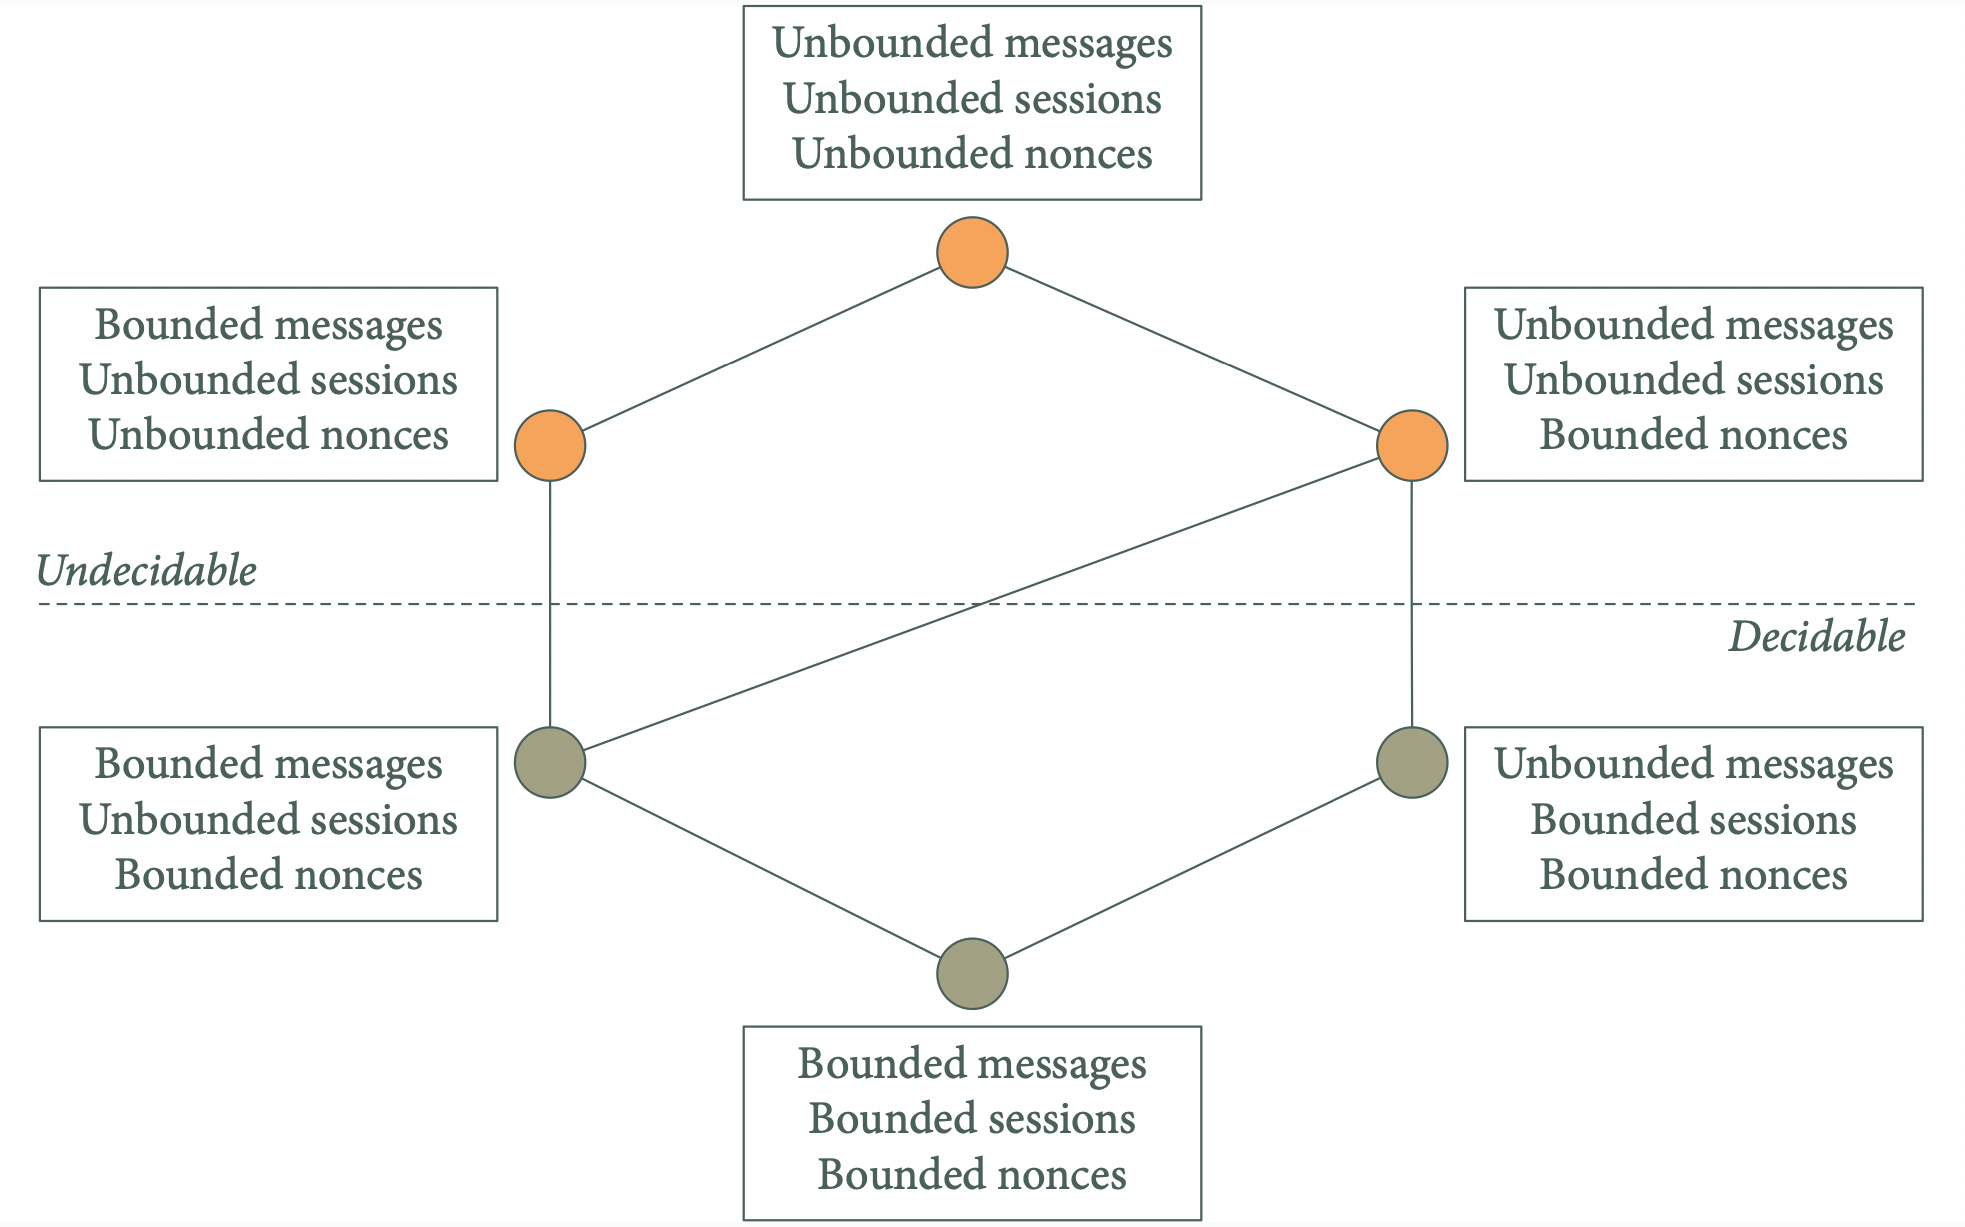
\includegraphics[width=0.8\textwidth]{Figures/undecidability.png}
    \caption{Decidability in symbolic verification. Image taken by N. Vitacolonna's presentation \cite{PresentazioneVitacolonna}}
\end{figure*}


In particular, as shown by N. Durgin et al. \cite{ComplexityOfBoundedSecurity}, by restricting different sources we can ensure to reduce the model checking problem to different complexity classes:

\begin{itemize}
    \item if we limit the number of nonces and messages, we end up with a DEXP-complete problem;
    \item if we restrict the number of sessions (and thus the number of nonces and messages), the problem will still be affected from unbounded state space, but its solution will be NP-complete; this workaround was adopted by a variety of tools such as Cl-AtSe \cite{clAtse}, OFMC \cite{ofmc} and SATMC \cite{satmc}.
\end{itemize}

Alternatively to bounding the sources of infinity, some software address undecidability by requiring human input (for example, Tamarin Prover \cite{tamarinIntroduction} features an interactive mode that allows the user to decide which security goals prioritize based on intermediate constraint systems, as we will see in \ref{subsec:tamarinGui}), returning inconclusive results (for example, ProverIf \cite{proverifIntroduction} may return an invalid attack trace) or even allowing non-termination.

\section{Tamarin Prover Overview}\label{sec:TamarinOverview}

In 2012, researchers at ETH introduced a new symbolic verification software, the Tamarin prover. Such tool provides an automated search for attacks, advanced protocol analysis techniques, and an interactive theorem proving approach that enables security experts to manually guide the proof process. We will now do a quick overview of its syntax, semantics and internal functioning; please refer to S. Meier's \cite{meierThesis} and B. Schmidt's \cite{schmidtThesis} PhD thesis and their introductory paper \cite{TamarinFoundations} for further information about the theoretical foundations regarding this tool, as long as its official manual \cite{tamarinManual} to solve any doubts about its use.

\subsection{Term algebra}

As explained in \ref{sec:SymbolicModel}, the Dolev-Yao model formalizes cryptographic messages within a term algebra; thus, in order to introduce Tamarin's syntax, we firsly have to take a look at (some) of the theoretical foundations behind the tool. 

\begin{definition}[Signature]
    A A signature $\Sigma$ is a finite set of functions of defined arity.
\end{definition}

Signatures are fundamental, since are the building blocks of our theory. As we will soon see, all the algebraic terms we introduced before (for example in equations \ref{eq:SymmetricEncryptionIdentity} and \ref{eq:AsymmetricEncryptionIdentity}) will be expressed as function symbols.

\begin{definition}[$\Sigma$-terms]
    G Given a signature $\Sigma$ and a set of variables $\chi$, with $\Sigma \cap \chi = \varnothing$ we can define the set of $\Sigma$-terms $\mathcal{T}_{\Sigma}(\chi)$ as the minimal set such as

    \begin{itemize}
        \item $\chi \subseteq \mathcal{T}_{\Sigma}(\chi)$
        \item $t_1,...,t_n \in \mathcal{T}_{\Sigma}(\chi) \land f/n \in \Sigma \implies f(t_1,...,t_n) \in \mathcal{T}_{\Sigma}(\chi)$
    \end{itemize}

    Note that $f/n$ indicates a function $f$ of arity $n$.
\end{definition}

While in this introduction we will deal with domain-agnostic logical terms, in practice Tamarin discriminates between 3 different types of terms to model various assumptions on different pieces of knowledge:

\begin{itemize}
    \item \textit{Fresh} (groud) terms are prefixed by a \textasciitilde{} and model information that we can assume a party can check for freshness.
    \item \textit{Public} names are juxtaposed by a \$ and formalize ground information that any party within the network knows.
    \item \textit{Normal} terms are any form of term: fresh, public or built upon function symbols.
\end{itemize}

$\Sigma$-terms allow us to recursively define algebraic terms starting from ground istances of variables. In real life we are able to combine multiple cryptographic primitives in order to build protocol messages: analogously, this set is made up of all the (countably infinite) possible combinations of function applications starting from ground terms.

Clearly, we need now a way to "compare" messages: as we previously explained in equations \ref{eq:SymmetricEncryptionIdentity} and \ref{eq:AsymmetricEncryptionIdentity}, the decryption of the encryption of any message (of course with the correct keys) must match the message itself. Similarly, all the primitives we will introduce must have some mechanism to check whether two terms belonging to a given set $\mathcal{T}_{\Sigma}(\chi)$ match each other or not.

\begin{definition}[Substitution]
    G Given a signature $\Sigma$ and a set of variables $\chi$, with $\Sigma \cap \chi = \varnothing$, a substitution is a function $\sigma: \chi \rightarrow \mathcal{T}_{\Sigma}(\chi)$.
\end{definition}

In our case, we do not only want to be able to build (and compare) terms upon ground instances of variables, but also build them upon other terms. As a consequence, we must generalize the definition of substitution:
    
\begin{definition}[Mapping]
    G Given a function $f/n \in \Sigma$, a mapping $\sigma':\mathcal{T}_{\Sigma}(\chi) \rightarrow \mathcal{T}_{\Sigma}(\chi)$ is an extension of a substitution $\sigma: \chi \rightarrow \mathcal{T}_{\Sigma}(\chi)$ such that
    \begin{equation*}
        f(t_1,...,t_n)\sigma' = f(t_1\sigma,...,t_n\sigma)
    \end{equation*}
\end{definition}

As we will soon see, mappings will be crucial for meaningful comparisons between terms. Of course, in our case we will narrow our focus on only sensible mappings that allow us to correctly model the cryptographic primitives needed. Each primitive will have a set of rules that will define its behaviour and such set will be formalized through equations:

\begin{definition}[Equation over $\Sigma$]
    G Given a signature $\Sigma$, a set of variables $\chi$, with $\Sigma \cap \chi = \varnothing$, an equation over $\Sigma$ is an unordered pair of terms $(t,u)$ with $t,u \in \mathcal{T}_{\Sigma}(\chi)$. Note that in this case, the equation would be written $t \simeq u$. In order to break loops while simplyfing terms, equations can be oriented (as $t \rightarrow u$).
\end{definition}

By introducing a set of equations $E$ we can create a congruence relation $=_E$ on terms $t$ and, consequently, equivalence classes $[t]_E$. The congruence relationship is known as an \textit{equational theory}. Introducing equational theories allows us to unify terms based on the quotient algebra $\mathcal{T}_{\Sigma}(\chi) /_{=_E}$: two terms $t,u \in \chi \cup \mathcal{T}_{\Sigma}(\chi)$ are equal in modulo $E$ if and only if they belong to the same class:
\begin{equation*}
    t =_E u \iff [t]_E = [u]_E
\end{equation*}

We will soon see how the use of equational theories enables us to formalize cryptographic primitives, but, before continuing, it is sensible to briefly talk about a decidability issue that regards this aspect of the term algebra.

\begin{definition}[$(\Sigma, E)$-Unification]
    G Given a signature $\Sigma$, a set of variables $\chi$, with $\Sigma \cap \chi = \varnothing$ and an equational theory $E$, two terms $t,u \in \mathcal{T}_{\Sigma}(\chi)$ are $(\Sigma,E)$-unifiable if there is at least a mapping $\sigma$ such that $t\sigma =_E u\sigma$.
\end{definition}

Normally, unification modulo theories is undecidable \cite{unificationUndecidability}: to overcome this issue Tamarin recommends users to only define \textit{subterm convergent theories} to ensure termination of the unification process \cite{subtermconvergent}. In practice, this constraint is never enforced by the tool, thus users must be careful when introducing custom theories (notice that exploiting only Tamarin's default equations overcomes this issue but may not be sufficient to model all the possible scenarios).

\begin{definition}[Convergent Theory]
    B Before defining what a convergent theory is, we have to define both \textit{terminating} and \textit{confluent} theories:

    \begin{itemize}
        \item A terminating theory is an equational theory which ensures that each term has a \textit{normal form} that can be reached through an arbitrary (but finite) number of substitutions.
        \item A confluent theory is an equational theory that ensures that if a term $t$ can be rewritten as both terms $t_1$ and $t_2$, then there must be a fourth term $t'$ that can be reached through an arbitrary number of substitutions from both $t_1$ and $t_2$.
    \end{itemize}

    A convergent theory is an equational theory that is both terminating and convergent.
\end{definition}

\begin{definition}[Subterm Convergent Theory]
    A A subterm convergent theory is an equational theory that is convergent and, for each equation $e: L \rightarrow R, e \in E$, $R$ is either ground and in normal form or a proper subterm of $L$.
\end{definition}

\subsection{Equational theories in Tamarin}

By default, Tamarin includes the function symbol \lstinline|*/2|, used in the \textit{AC-equational theory}:
\begin{align*}
    x * (y * z) &\simeq (x * y) * z\ \ \textrm{(associativity)}\\
    x * y &\simeq y * z\ \ \textrm{(commutativity)}
\end{align*}

This theory clearly models some properties of multiplication. Similarly, the tool provides function symbols (\lstinline|pair/2|, \lstinline|fst/1| and \lstinline|snd/1|) and equations to work with pairs: 
\begin{align*}
    fst(pair(x,y)) &\simeq x\\
    snd(pair(x,y)) &\simeq y
\end{align*}

Other function symbols are shipped within the tool, but must be loaded into a theory through the \lstinline|built-ins| directive:

\paragraph{hashing}
The \lstinline|hashing| theory defines the symbol \lstinline|h/1| and no equations. This clearly models the one-wayness of an ideal hash function, which cannot be reversed (the only way to determine whether the pre-image of \lstinline|h(x)| is \lstinline|x| is to find \lstinline|x|).

\paragraph{symmetric encryption}
The \lstinline|symmetric-encryption| theory models equation \ref{eq:SymmetricEncryptionIdentity} in a very natural way: after providing symbols \lstinline|senc/2| and \lstinline|sdec/2|, it defines the equation
\begin{equation*}
    sdec(senc(m,k),k) = m
\end{equation*}
which enforces the fact that the only way to access an encrypted term is to know the decryption key (perfect cryptography assumptions).

\paragraph{asymmetric encryption}
Similarly to last paragraph, the \lstinline|asymmetric-encryption| theory formalizes equation \ref{eq:AsymmetricEncryptionIdentity} through symbols \lstinline|pk/1|, \lstinline|aenc/2| and \lstinline|adec/2| and the equation
\begin{equation*}
    adec(aenc(m, pk(sk)), sk) = m
\end{equation*}
By not providing other equations, this ensures that an attacker is not able neither to decrypt an encrypted message without the private secret, nor to deduce a private key from it corrispondent public counterpart.

\paragraph{signing}
The \lstinline|signing| theory allows to model digital signing schemes. It introduces symbols \lstinline|sign/2|, \lstinline|verify/3|, \lstinline|pk/1|, \lstinline|true/0| and the equation
\begin{equation*}
    verify(sign(m,sk), m, pk(sk)) = true
\end{equation*}
Yet again, not providing other equations enforces the fact that the attacker is not able to forge valid signatures without first finding a private key.

\paragraph{diffie hellman}
Perhaps the most complex built-in theory is the \lstinline|diffie-hellman| one: it defines function symbols \lstinline|inv/1|, \lstinline|1/0|, \lstinline|^/2| and \lstinline|*/2| and the following equations:
\begin{align*}
    (x^y)^z  &\simeq x^{(y*z)}\\
    x^1      &\simeq x\\
    x*y      &\simeq y*x\\
    (x*y)*z  &\simeq x*(y*z)\\
    x*1      &\simeq x\\
    x*inv(x) &\simeq 1
\end{align*}
Note that this theory allows to effectively model Diffie Hellman exchanges (both classical and with elliptic curves) while providing the remaining multiplication properties not captured by the AC theory (namely the inverse and the identity).

\paragraph{Other built-in theories}
There are other built-in theories that can be included within a Tamarin model:

\begin{enumerate}
    \item \lstinline|revealing-signing|
    \item \lstinline|bilinear-pairing|
    \item \lstinline|xor|
    \item \lstinline|multiset|
    \item \lstinline|reliable-channel|
\end{enumerate}

for the sake of brevity we will not introduce them, but we encourage any interested reader into looking at their definitions within the manual \cite{tamarinManual}.

\paragraph{User-defined theories}
Furthermore, a user can define additional custom theories to model any cryptographic primitive or mechanism required for a security protocol.

For example, one may want to model the homomorphic properties of a symmetric encryption scheme (for example vanilla RSA's invariance under multiplication): to do so, it is sufficient to add the following equation to a formalization after the \lstinline|equations| keyword (of course assuming the relative built-in theories have already been included):
\begin{equation*}
    aenc(m1, k) * aenc(m2, k) \simeq aenc(m1*m2, k)
\end{equation*}

Similarly, when dealing with elliptic curve cryptography, it is possible to use the same keypair both for the Ed25519 signing schema and the X25519 exchange procedure \cite{signdh}. Such behaviour can be modeled by introducing the following equation \footnote{Note that this is not entirely true: name clashing on symbols may force the user to rename some functions for this to work. In any case, it is possible to simply avoid including the built-ins and explicitly defining the relative equational theories following the definitions introduced in this section without using reserved names.} (again, considering the \lstinline|diffie-hellman| and \lstinline|asymmetric-encryption| built-ins as already included):
\begin{equation*}
    g^x \simeq pk(x)
\end{equation*}
where $g$ is a public constant symbolizing the generator of the curve.

Finally, it has to be noted that a custom symbol can be defined with the \lstinline|[private]| keyword to prevent the attacker from creating new terms with it. This could be useful if, for example, we wanted to model a protocol in which there is a cryptographic primitive (like a secret hash function) that, for some reason, is accessible only by the intended parties of an exchange. It is well know that "security by obscurity" is not a principle to follow at all, but this attribute makes the formalization of similar contexts straightforward. All the other functions are considered public and thus can be employed by the user and the attacker alike.

\subsection{Formalizing protocols as sets of rewriting rules}

In Tamarin, the execution of a protocol is modeled by the evolution of a multiset of facts. In knowledge representation, facts are "true" predicates that have a fixed arity and are composed of terms; Tamarin follows this definition and requires the user to define them with a starting capital letter and provides two different versions of them:

\begin{itemize}
    \item \textit{linear facts} can be consumed only once and are useful to model state transitions and ephemeral messages;
    \item \textit{persistent facts} can be consumed unlimited times and are optimal to model enduring knowledge (and are syntatically prefixed by an exclamation mark).
\end{itemize}

Tamarin allows protocol (and adversary) modeling through multiset rewriting rules.

\begin{definition}[Labelled rewriting rule]

Given a multiset $\Gamma_t = \{ F_0, ..., F_n \}$ and a sequence of multisets $trace_t = \langle a_0, ..., a_{t-1} \rangle$ at a time $t$, we can define a rewrite rule as a triple of multisets $RR = \langle L, A, R \rangle$ (written as $RR= L -[ A ] \rightarrow R$) such that:

\begin{itemize}
    \item we can apply $RR$ to $\Gamma_t$ if there is at least one ground instance (i.e. an instance with no variables) $rr = l -[ a ] \rightarrow r$ of $RR$ so that $l \subseteq^{\#} \Gamma_t$
    \item applying $rr$ to $\Gamma_t$ yields to a new state $\Gamma_{t+1}$ and an increased trace $trace_{t+1}$ obtained as
\begin{align*}
    \Gamma_{t+1} &= \Gamma_t \setminus^{\#} lin(l) \cup^{\#} r\\
    trace_{t+1} &= \langle a_0, ..., a_{t-1}, a \rangle
\end{align*}
\end{itemize}
in which $\setminus^{\#}$ and $\cup^{\#}$ are the multiset equivalent operations for set difference and union and $lin(l)$ is the multiset of linear facts belonging to $l$ (notice that persistent facts are never removed from the state). From now on, we will refer to $L$, $R$ and $A$ as the multisets of \textit{premises}, \textit{conclusions} and \textit{action facts} of a rule (in this order). 

Note that each rule is labelled by a name $N$, thus can be seen as a pair $(N, RR)$
\end{definition}

Notice the detail about the trace being a sequence and not a set: since security properties will be later on specified as guarded fragments of first order temporal logic on set of traces, the ordering relation present in a sequence allows to define temporal relations between different action facts.

In particular, given a set of rewriting rules $P$, Tamarin will analyze the set of all the possible traces generated by executions of P:

\begin{definition}[Set of possible traces]
    G Given a set of labelled rewriting rules $P = \{(N_1,RR_1),...,(N_m,RR_m)\}$, we define the set of possible traces generated by $P$ as
    \begin{align*}
        traces(P) = \{ &\langle A_1,...,A_n \rangle |\\
        & \exists S_1,...,S_n . \varnothing ^{\#} \xrightarrow[]{A_1} S_1 \xrightarrow[]{A_2} ... \xrightarrow[]{A_n} S_n\\
        & \textrm{and no ground istance of } Fresh()\\
        & \textrm{is used twice }\}
    \end{align*}
    where $A_i$ is $RR_i$'s action facts multiset.
\end{definition}

Furthermore, it is important to note that security properties will be specified on specific types of traces, namely \textit{observable traces}.

\begin{definition}[Observable trace]
    G Given a trace $tr$, we can compute its relative observable trace $tr_{obs}$ by removing all the empty multisets from it:
    \begin{equation*}
        tr_{obs} = \langle A_i | A_i \in tr \land A_i \neq \varnothing^{\#} \rangle
    \end{equation*}
\end{definition}

To better understand how such trace (both observable and non) is derived from a protocol's execution, we can take a look at the following example rewriting system:
\begin{align*}
    P = \{ &(N_1, \varnothing^{\#}-[\{\{\textrm{Init}(0)\}\}] \rightarrow \{\{A(0)\}\}),\\
    &(N_2, \{\{A(x)\}\}-[\varnothing^{\#}] \rightarrow \{\{B(x)\}\})\\
    &(N_3, \{\{B(x)\}\}-[\{\{\textrm{Concl}(x)\}\}] \rightarrow \varnothing^{\#})\}
\end{align*}

Let us assume we are starting with an empty state $\Gamma_0$ and apply rules $N_1, N_2, N_1, N_3$, in this order. The state would evolve as:
\begin{align*}
    \Gamma_0 &= \varnothing^{\#} \setminus^{\#} \varnothing^{\#} \cup^{\#} \{\{A(0)\}\} = \{\{A(0)\}\}\\
    \Gamma_1 &= \{\{A(0)\}\} \setminus^{\#} \{\{A(0)\}\} \cup^{\#} \{\{B(0)\}\} = \{\{B(0)\}\}\\
    \Gamma_2 &= \{\{B(0)\}\} \setminus^{\#} \varnothing^{\#} \cup^{\#} \{\{A(0)\}\} = \{\{A(0), B(0)\}\}\\
    \Gamma_3 &= \{\{A(0), B(0)\}\} \setminus^{\#} \{\{B(0)\}\} \cup^{\#} \varnothing^{\#} = \{\{A(0)\}\}
\end{align*}
while the generated trace would be
\begin{equation*}
    tr = \langle \{\{\textrm{Init}(0)\}\}, \{\{\varnothing^{\#}\}\}, \{\{\textrm{Init}(0)\}\}, \{\{\textrm{Concl}(0)\}\},\rangle
\end{equation*}
and the observable trace
\begin{equation*}
    tr_{obs} = \langle \{\{\textrm{Init}(0)\}\}, \{\{\textrm{Init}(0)\}\}, \{\{\textrm{Concl}(0)\}\}\rangle
\end{equation*}

\subsubsection{Dolev Yao rules}
Although the above described multiset rule rewriting system can be used for general model checking, Tamarin provides a set of built-in rules to model connections within Dolev-Yao's adversary controlled network:

\begin{itemize}
    \item \lstinline|[] --[]-> [ Fr(~msg) ]| allows for the generation of new fresh values.
    \item \lstinline|[ Fr(~msg) ] --[]-> [ K(~msg) ]| allows for the generation of new fresh values by the attacker.
    \item \lstinline|[ Out(msg) ] --[]-> [ K(msg) ]| allows the attacker to eavesdrop all messages travelling through the network. 
    \item \lstinline|[ K(msg) ] --[ K(msg) ]-> [ In(msg) ]| allows user to retrieve messages from the attacker-controlled network.
    \item \lstinline|[] --[]-> [ K($x) ]| allows the attacker to discover all public names.
    \item \lstinline|[ K(x1,...,xn) ] --[]-> [ K(f(x1,...,xn)) ]| allows the attacker to apply $n$-ary functions to arguments he already knows.
\end{itemize}

Notice that these rule allow us to easily specify security properties about the knowledge of the attacker (for example, confidentiality): if we wanted to ensure that a protocol does not reveal a certain secret \lstinline|sec|, we just need to require that \lstinline|K(sec)| does not appear within any of the multisets of the observable trace.

Tamarin only provides built-in facts for communication over insecure and reliable channels, but if we needed to formalize other types of connections we could use the above rule as a blueprint to define them. For example, to model a confidential channel (thus a connection in which the attacker could send, but not read from messages), one may define the following rules:

\begin{lstlisting}[language=Tamarin]
rule Send_Over_Confidential_Channel :
    [ ConfOut(msg) ]
    --[]->
    [ ConfIn(msg) ]

rule Attacker_Sends_Over_ConfChannel :
    [ K(msg) ]
    --[]->
    [ ConfIn(msg) ]
\end{lstlisting}

As we can see, there is no rule that allows the adversary to learn anything from the confidential channel, but he might send any forged message through it. On the other hand, an honest user could employ the \lstinline|ConfOut| and \lstinline|ConfIn| facts to model sending and retrieval on the channel. Possibly, if we wanted, we could also differentiate between channels by augmenting the rules with a connection identifier:

\begin{lstlisting}[language=Tamarin]
rule Send_Over_Confidential_Channel :
    [ ConfOut(msg, channel) ]
    --[]->
    [ ConfIn(msg, channel) ]

rule Attacker_Sends_Over_ConfChannel :
    [ K(msg), K(channel) ]
    --[]->
    [ ConfIn(msg, channel) ]
\end{lstlisting}

Similarly, to model an authentic channel (a connection where integrity, but not confidentiality is guaranteed), we could define the following rule:

\begin{lstlisting}[language=Tamarin]
rule Send_Over_Authentic_Channel :
    [ AuthOut(msg) ]
    --[ K(msg) ]->
    [ AuthIn(msg), K(msg) ]
\end{lstlisting}

By not including a rule that allows the attacker to produce \lstinline|AuthOut| or \lstinline|AuthIn| facts, we ensure that such channel cannot be polluted with forged messages. Again, we could trivially differentiate between channels or build both confidential and authentic (secure) connections with analogous rules.

\subsection{Trace properties}\label{subsec:TraceProperties}

As previously anticipated, in Tamarin security properties are expressed as guarded fragments of first order logic. The keyword adopted by Tamarin to indicate a property to prove is \lstinline|lemma|. Lemmas can be either of type \lstinline|exists-trace|, which are demonstrated by finding a single valid protocol trace verifing the formula, or \lstinline|all-traces|, which are proved by negating the property and trying to find a counterexample. To specify a lemma, we can combinate the following atoms:

\begin{itemize}
    \item false $\bot$;
    \item logical operators $\neg\  \wedge\  \vee\ \implies$;
    \item quantifiers and variables $\forall\ \exists\ a\ b\ c$;
    \item term equality $t_1 \approx t_2$;
    \item time point ordering and equality $i < j$ and $i = j$;
    \item action facts at time points $F @ i$ (for an action fact $F$ at timepoint $i$).
\end{itemize}

Keeping in consideration that also properties can define sets of traces similarly to protocol rules, we can define correctness as follows:

\begin{definition}[Correctness]
    G Given a set of protocol rules $P$ and a property to prove $\phi$, $P$ is correct in regards to $\phi$ if and only if the set of traces generated by $P$ is a subset of the one generated by $\phi$:
    \begin{equation*}
        P \vDash \phi \iff traces(\phi) \subseteq traces(P)
    \end{equation*}

    On the contrary, if $P \nvDash \phi$, all traces belonging to $traces(P) / traces(\phi)$ represent valid attacks.
\end{definition}

Note that property proving is done by Tamarin through \textit{constraint systems} resolving. In turn, these systems are simplified by executing a backwards search within the relative protocol's \textit{dependencies graph} (a graph that, for each fact used by a Tamarin \textit{theory}, describes the list of possible rules usable to obtain it). The theoretical foundations behind property proving are beyond the scope of this report, but are explained in detail in \cite{schmidtThesis} \cite{meierThesis}. As end users, we can be satisfied by knowing that Tamarin's verification algorithm, although does not guarantee termination, is both \textit{sound} and \textit{complete} \cite{schmidtThesis} \cite{meierThesis} \cite{xorCompleteness}.

\subsection{Observational equivalence properties}\label{subsec:ObsEqProperties}

When operated in \textit{Observational Equivalence Mode} (refer to the official documentation \cite{tamarinManual} for further reference), Tamarin allows for the use of the \lstinline|diff/2| operator \cite{tamarinObsEquivalences}, that permits to demonstrate \textit{diff equivalence} properties. To understand what a diff equivalence property is, we have to firstly introduce the concept of \textit{trace equivalence}

\begin{definition}[Trace equivalence]
    Two different protocols $P_1, P_2$ are trace equivalent if and only if for each trace of $P_1$ exists a trace of $P_2$ so that the messages exchanged during the two executions are indistinguishable.
\end{definition}

This is the weakest (and thus most suitable for security verification) form of observational equivalence. Since many problems in this category are undecidable in nature \cite{traceObservableProperties}, Tamarin only allows diff equivalences in aid of termination.

\begin{definition}[Diff equivalence]
    Two protocols $P_1, P_2$ are diff-equivalent if and only if they have the same structure and differ only by the messages exchanged.

    Thus, the two protocol have the same structure during execution.
\end{definition}

The previously introduced \lstinline|diff(left, right)| operator allows to define a protocol rule that can be instantiated either with the \lstinline|left| or \lstinline|right| value. For each one of them, Tamarin constructs the relative dependencies graph and checks if they are equivalent, which is a sufficient criterion for observational diff-equivalence. Please note that a formal definition of \textit{dependencies graph equivalence}, along with the subsequent demonstration of sufficiency are available in the introductory paper for the observational equivalences in Tamarin written by D. Basin, J. Dreier and R. Sasse \cite{tamarinObsEquivalences}.

\subsection{Aiding termination}

Since protocol verification is an inherently undecidable problem, Tamarin provides some additional functionalities engineered to aid termination.

\subsubsection{Source lemmas}

As explained before, Tamarin elaborates the dependencies graph related to a theory before beginning constraint solving. Since the prover uses an untyped system, in certain cases it is not able to deduce the source of one or more facts, causing partial deconstructions. As explained by V. Cortier \cite{autosources}, for example, this situation occurs whenever the same message has to travel across the network multiple times. To mitigate this issue, Tamarin allows to define a lemma with the additional tag \lstinline|[sources]|, which is automatically proved during the precomputation phase and allows to declare the origin of one or more messages.

An example of this type of lemma, along with its explanation, will be provided in section \ref{subsec:termination}

Note that V. Cortier, S. Dealune and J. Dreier proposed an algorithm for automatic source lemma generation \cite{autosources} that has already been integrated in Tamarin (run the program with the additional \lstinline|--auto-sources| tag to execute the extension), but sometimes it leads to non-termination during the precomputation phase.

\subsubsection{Oracles}

During constraint-solving, Tamarin uses its built-in \textit{smart} heuristic (refer to the relevant section of the manual \cite{tamarinManual} for further reference) to sort the list of security goals to check. Sometimes, though, the algorithm prioritizes the wrong goals, leading to loops in the search and thus to non-termination. In an attempt to prevent this behavior, Tamarin provides also two variants of the \textit{consecutive} heuristic, which guarantee to avoid delaying any goal infinitely to exclude starvation. This causes bigger proofs and still fails to solve the problem sometimes.

By knowing how to manually guide the search (for example after doing some practice with the built-in interactive mode), we can code (in any programming language of choice) an external \textit{oracle}, which will be automatically run by the prover to determine the right priority objective to solve within a list of current goals. This user-defined software receives the name of the lemma and the indexed goal list (sorted by the smart heuristic) as input, and returns the re-ranked list (or, alternatively, only its first element) as output. Note that oracles are generally stateless: for each step of the proof, the program is executed from scratch, with only the name of the considered lemma and the list of current security goals as input.

\subsubsection{Interactive mode}\label{subsec:tamarinGui}

The Tamarin interactive mode is a powerful feature that enables users to guide the proof search process and interactively inspect the demonstration as it is being constructed. When using the interactive mode, users can provide hints and guidance to the Tamarin prover, which can significantly speed up the proof search process and help to identify any potential issues or vulnerabilities in the security protocol being analyzed. For example, by interleaving automatic steps and manual selection of goals to solve, the user can understand if the tool is entering an infine loop of computation or not by monitoring wheter recursive structures of terms are being produced or not. Furthermore, by guiding the proof, the user can easily guess how to build an effective oracle to speed up lenghty proofs. Additionally, the interactive mode provides a valuable opportunity to gain a deeper understanding of how the Tamarin prover works and how it constructs proofs for security protocols. An example of Tamarin in action in interactive mode is displayed in figure \ref{fig:interactive}.

\begin{figure*}
    \centering
    \captionsetup{justification=centering, margin=1cm}
    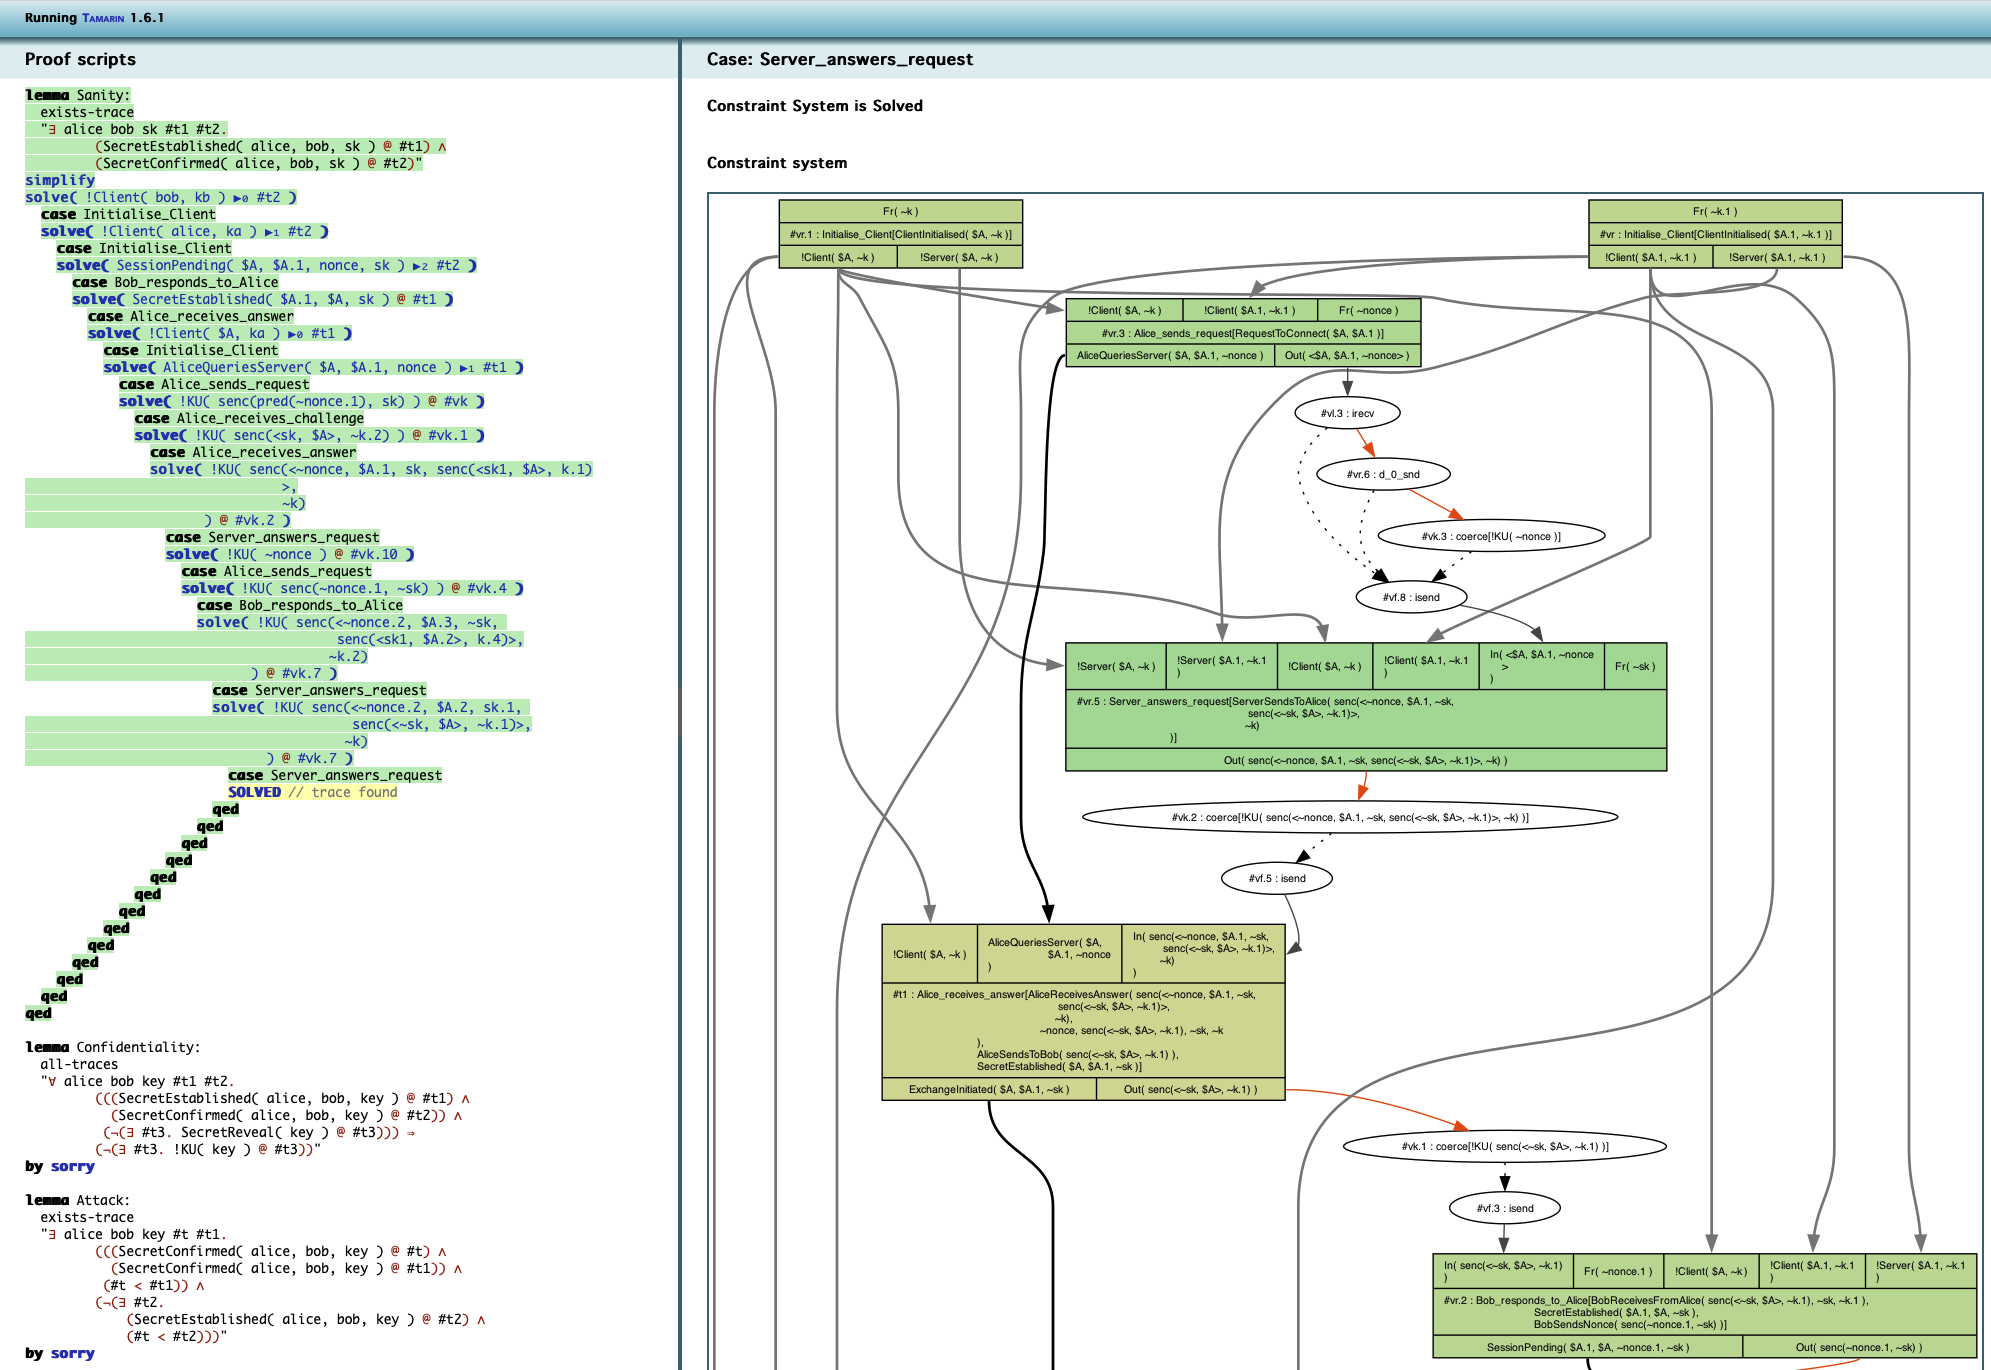
\includegraphics[width=0.8\textwidth]{Figures/gui.png}
    \caption{Tamarin's interactive mode}
    \label{fig:interactive}
\end{figure*}

\subsubsection{Restrictions}

Similarly to lemmas, \textit{restrictions} are specified through guarded fragments of first order logic. The difference between the two is that while lemmas express properties to prove, a restriction limits the possible traces of a protocol to the executions that satisfy the specified formula. An example of restriction use could be to avoid the application of the same rule twice:

\begin{lstlisting}[language=Tamarin]
rule Generic_rule :
    [ OldFact(x) ]
    --[ OnlyOnce() ]->
    [ NewFact(x) ]

restriction Do_not_repeat :
    "All #i #j .
        OnlyOnce() @ #i &
        OnlyOnce() @ #j
            ==> #i = #j"
\end{lstlisting}

\subsubsection{Re-use lemmas}

Finally, the last functionality we introduce are \textit{re-use lemmas}: defined with the \lstinline|[reuse]| keyword, these formulas, once proved, can be used by Tamarin in the demonstration of the subsequent specified lemmas.

\section{The Needham-Schroeder Protocol}

The Needham-Schroeder protocol is a key exchange protocol that was introduced in 1978 by Roger Needham and Michael Schroeder \cite{needhamschroeder} to address the issue of authentication in distributed computer networks using symmetric key cryptography.

The Needham-Schroeder protocol is used to establish a shared symmetric key between two parties in a networked environment. The exchange assumes that both parties already have a shared secret with a trusted third party, referred to as a key distribution center (KDC). The KDC is responsible for generating and distributing secret keys to each party, and it also has a public key that can be used to verify the authenticity of messages sent by the KDC.

In the Needham-Schroeder protocol, when one party (Alice) wants to communicate securely with another party (Bob), she sends a request to the KDC for a session key to use in the communication. The KDC then generates a new session key and sends it to Alice encrypted using Bob's public key. Alice can then decrypt the session key using her shared secret with the KDC, and use it to communicate with Bob.

The protocol also includes a mechanism for mutual authentication, which ensures that each party is who they claim to be. When Alice receives the session key from the KDC, she sends a message to Bob that includes the session key and a nonce (a random number). Bob then encrypts the nonce with the session key and sends it back to Alice. Alice can then decrypt the message and verify that the nonce matches the one she sent to Bob. This process ensures that both parties have successfully authenticated each other, and they can begin communicating securely using the session key. The exchange is summarized in diagram \ref{fig:NS}.

\begin{figure}[h]
    \centering
    \captionsetup{justification=centering, margin=1cm}
    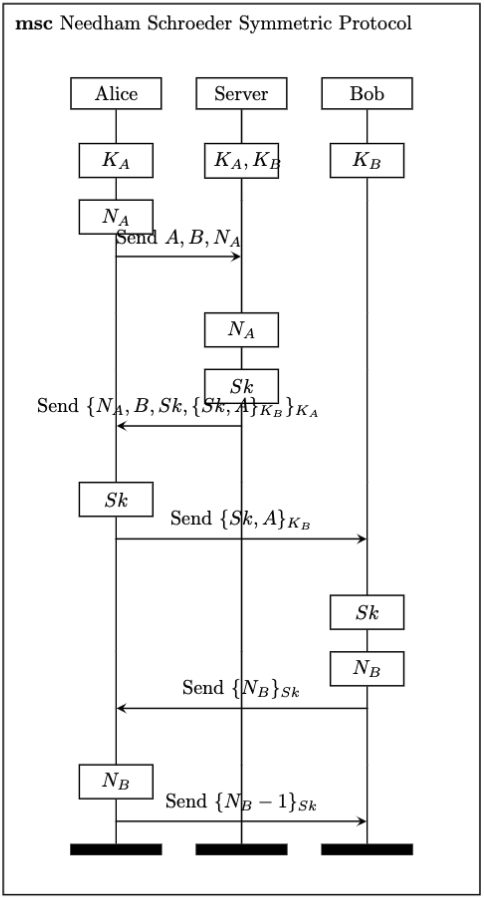
\includegraphics[width=0.45\textwidth]{Figures/NS.png}
    \label{fig:NS}
    \caption{Needham-Schroeder Symmetric protocol}
\end{figure}
%\begin{msc}{Needham Schroeder Symmetric Protocol}
    \declinst{alice}{}{Alice}
    \declinst{server}{}{Server}
    \declinst{bob}{}{Bob}
    \action*{ \begin{minipage}{1cm}\centering $K_A$ \end{minipage} }{alice}
    \action*{ \begin{minipage}{1cm}\centering $K_A, K_B$ \end{minipage} }{server}
    \action*{ \begin{minipage}{1cm}\centering $K_B$ \end{minipage} }{bob}
    \nextlevel[2]
    \action*{ \begin{minipage}{1cm}\centering $N_A$ \end{minipage} }{alice}
    \nextlevel[2]
    \mess{Send $A, B, N_A$}{alice}{server}
    \nextlevel[2]
    \action*{ \begin{minipage}{1cm}\centering $N_A$ \end{minipage} }{server}
    \nextlevel[2]
    \action*{ \begin{minipage}{1cm}\centering $Sk$ \end{minipage} }{server}
    \nextlevel[2]
    \mess{Send $\{N_A, B, Sk, \{Sk, A\}_{K_B} \}_{K_A}$}{server}{alice}
    \nextlevel[2]
    \action*{ \begin{minipage}{1cm}\centering $Sk$ \end{minipage} }{alice}
    \nextlevel[2]
    \mess{Send $\{Sk, A\}_{K_B}$}{alice}{bob}
    \nextlevel[2]
    \action*{ \begin{minipage}{1cm}\centering $Sk$ \end{minipage} }{bob}
    \nextlevel[2]
    \action*{ \begin{minipage}{1cm}\centering $N_B$ \end{minipage} }{bob}
    \nextlevel[2]
    \mess{Send $\{N_B\}_{Sk}$}{bob}{alice}
    \nextlevel[2]
    \action*{ \begin{minipage}{1cm}\centering $N_B$ \end{minipage} }{alice}
    \nextlevel[2]
    \mess{Send $\{N_B-1\}_{Sk}$}{alice}{bob}
\end{msc}

While the Needham-Schroeder protocol is widely used in computer security, it is not without its flaws. One issue is the potential for a "replay attack," where an attacker intercepts and reuses a previously transmitted message to gain access to the network. Another issue is the reliance on a trusted third party, which can be a single point of failure if compromised.

To address these issues, Needham and Schroeder later extended their protocol to include public-key cryptography, resulting in the Needham-Schroeder Public-Key Protocol. This protocol addressed the weaknesses of the original protocol by using public-key cryptography to establish the authenticity of each party's public key and ensure the confidentiality and integrity of the communication.

\subsection{Tamarin Formalization}

\subsubsection{The protocol}

Formalizing the Needham-Schroeder exchange in Tamarin is quite straightforward thanks to the built-in functions and simple syntax provided by the tool (note that all the source files of this section are available for local verification at \cite{github}).

\paragraph{Initialisation}

The clients (Alice and Bob) and the server are initialised with the shared secrets through the following rule:

\begin{lstlisting}[language=Tamarin]
rule Initialise_Client :
    [
        Fr(~k)
    ]
    --[ ClientInitialised($A, ~k) ]->
    [
        !Client($A, ~k),
        !Server($A, ~k$)
    ]
\end{lstlisting}

Note that since we do not have any particular reason to believe that identities are private, we must formalize them as public names known to the attacker. To avoid that the same client gets instantiated twice with two different keys, we exploit the \lstinline|ClientInitialised| action-fact in the following restriction:

\begin{lstlisting}[language=Tamarin]
restriction EachClientCanBeInitialisedOnce :
    "All client key1 key2 #t1 #t2 .
        ClientInitialised(client, key1) @ #t1 &
        ClientInitialised(client, key2) @ #t2
            ==> #t1 = #t2"
\end{lstlisting}

\paragraph{$A \to S: A,B,N_A$}

The first message sent by Alice to initiate the protocol is easily modelled through the following rule (and restriction):

\begin{lstlisting}[language=Tamarin]
rule Alice_sends_request :
    [
        !Client(alice, ka),
        !Client(bob, kb),
        Fr(~nonce)
    ]
    --[ RequestToConnect(alice, bob) ]->
    [
        AliceQueriesServer(alice, bob, ~nonce),
        Out(<alice, bob, ~nonce>)
    ]

restriction NoSelfCommunication:
    "All client #t .
        RequestToConnect(client, client) @ #t ==> F"
\end{lstlisting}

There are multiple elements that we should analyze within this snippet:

\begin{itemize}
    \item The restriction \lstinline|NoSelfCommunication| exploits the \lstinline|RequestToConnect| action fact to restrict connections to only different parties. This is done to prevent Tamarin to waste resources in analyzing self-communicating runs of the protocol, which would be useless in a key-exchange scenario.
    \item This rule also models the generation of the nonce $N_A$.
    \item The fact \lstinline|AliceQueriesServer| will then be useful, once Alice will receive the server's response, to ensure that she was actually the one which initiated the protocol with a fresh nonce before.
\end{itemize}

\paragraph{$S \to A: \{N_A, B, Sk, \{Sk, A\}_{K_B} \}_{K_A}$}

Similarly, the role of the server in the exchange can be modelled through a single rule:

\begin{lstlisting}[language=Tamarin]
rule Server_answers_request :
    let
        message_to_bob = senc(<~sk, alice>, kb)
        message_to_alice = senc(<nonce, bob, ~sk, message_to_bob>, ka)
    in
    [
        !Server(alice, ka),
        !Server(bob, kb),
        !Client(alice, ka),
        !Client(bob, kb),
        In(<alice, bob, nonce>),
        Fr(~sk)
    ]
    --[ ServerSendsToAlice(message_to_alice) ]->
    [
        Out(message_to_alice)
    ]
\end{lstlisting}

Here we exploit the symbolic function primitive \lstinline|senc| included in the built-in \lstinline|symmetric-encryption| equational theory to model the encrypting procedure executed by the server. The action-fact \lstinline|ServerSendsToAlice| will be later used within a source lemma to solve Tamarin's partial deconstruction problem within this theory.

\paragraph{$A \to B: \{Sk, A\}_{K_B}$}

Here we formalize the message sent from Alice to Bob containing the shared secret key generated by the server.

\begin{lstlisting}[language=Tamarin]
rule Alice_receives_answer :
    let
        message_to_bob = senc(<sk1, alice>, k)
        message_to_alice = senc(<nonce, bob, sk, message_to_bob>, ka)
    in
    [
        !Client(alice, ka),
        AliceQueriesServer(alice, bob, nonce),
        In(message_to_alice)
    ]
    --[ AliceReceivesAnswer(message_to_alice, nonce, message_to_bob, sk, ka),
        AliceSendsToBob(message_to_bob),
        SecretEstablished(alice, bob, sk) ]->
    [
        ExchangeInitiated(alice, bob, sk),
        Out(message_to_bob)
    ]
\end{lstlisting}

Similarly to before, the \lstinline|AliceQueriesServer| fact is consumed to produce an analogous \lstinline|ExchangeInitiated| fact, that will be later on used to keep a copy of the shared key and to ensure that Alice actually initiated an exchange if the subsequent messages will come through.

Note that, due to Tamarin's ability to manage an unbounded number of messages, here we had to take a little shortcut in the formalization to force termination during proofs: Alice is not actually able to check the content of the \lstinline|message_to_bob|, since she does not have a copy of his private key $K_B$, but here we use pattern matching to ensure that at least her identity is part of a message structured according the protocol specification. This assumption does not allow us to prove the security properties of the protocol without a little loss of generality, but it is crucial to avoid that Tamarin tries to find an attack trace with an infinite nested sequences of messages. Note that we did not enforce any pattern matching on $K_B$ and $Sk$ to avoid taking any further assumption.

Again, the \lstinline|AliceReceivesAnswer| and |AliceSendsToBob| action-facts will be exploited in the final sources lemma, while \lstinline|SecretEstablished| will be useful to specify the security properties later on.

\paragraph{$B \to A: \{N_B\}_{Sk}$}

Now we can model the challenge of Bob to Alice:

\begin{lstlisting}[language=Tamarin]
rule Bob_responds_to_Alice :
    let
        message_from_alice = senc(<sk, alice>, kb)
        encrypted_nonce = senc(~nonce, sk)
    in
    [
        In(message_from_alice),
        Fr(~nonce),
        !Client(alice, ka),
        !Client(bob, kb),
        !Server(bob, kb)
    ]
    --[ BobReceivesFromAlice(message_from_alice, sk, kb),
        SecretEstablished(bob, alice, sk),
        BobSendsNonce(encrypted_nonce) ]->
    [
        SessionPending(bob, alice, ~nonce, sk),
        Out(encrypted_nonce)
    ]
\end{lstlisting}

Following the structure of the previous rules, we can see that the formalization of this part of the exchange is pretty straightforward. The \lstinline|SessionPending| fact is useful to keep track of the run of the protocol from the point of view of Bob, while the \lstinline|BobReceivesFromAlice| and \lstinline|BobSendsNonce| action fact are necessary to ensure solving partial deconstructions. Finally, this \lstinline|SecretEstablished| fact will be used to specify a "sanity check" of the protocol via an \lstinline|exists-trace| lemma.

\paragraph{$A \to B: \{N_B - 1\}$}

We still need to formalize the last exchange. In order to model the answer to Bob's challenge, we need to define a custom function to have the predecessor function at our disposal within the theory: the following snippet will provide both such definition (that, due to Tamarin's syntax will be kept at the top of the file) and the subsequent rule for formalizing this step of the protocol.

\begin{lstlisting}[language=Tamarin]
function: pred/1

rule Alice_receives_challenge :
    let
        nonce_received = senc(nonce, sk)
        nonce_sent = senc(pred(nonce), sk)
    in
    [
        !Client(alice, ka),
        ExchangeInitiated(alice, bob, sk),
        !Client(bob, kb),
        In(nonce_received)
    ]
    --[ AliceReceivesNonce(nonce_received, nonce, sk) ,
        AliceSendsNonce(nonce_sent)]->
    [
        !Session(alice, bob, sk),
        Out(nonce_sent)
    ]
\end{lstlisting}

Again, if we modeled both the predecessor and the successor function, the theory would become indecidable and the security properties would not be unprovable since Tamarin would get stuck while trying to build infinite sequences of predecessors and successors.

Note that within the premises of this rule we consume the fact \lstinline|ExchangeInitiated| to replace it with a persistent \lstinline|!Session| between Alice and Bob. The action facts contained in the previous snippet will allow us to specify (yet again) the source lemma.

\paragraph{Conclusion}

The last protocol rule enable us to formalize the establishment of the session from Bob's perspective:

\begin{lstlisting}[language=Tamarin]
rule Bob_receives_challenge_answer :
    let
        received_nonce = senc(pred(nonce), sk)
    in
    [
        !Client(bob, kb),
        !Client(alice, ka),
        SessionPending(bob, alice, nonce, sk),
        In(received_nonce)
    ]
    --[ BobReceivesNonce(received_nonce, nonce, sk),
        SecretConfirmed(alice, bob, sk) ]->
    [
        !Session(bob, alice, sk)
    ]
\end{lstlisting}

Note the use of pattern matching to enforce the fact that Alice (or the attacker) must send the predecessor of the nonce previously communicated in order to trigger this transition. The \lstinline|SecretConfirmed| action-fact will be required to specify the end of the execution in the following lemmas, while \lstinline|BobReceivesNonce| will be part of the source lemma.

\paragraph{Modelling the attacker}

Soon we will provide an example of a possible attack to the protocol, but to do so we first need to give to the attacker the capability of deducing a previously used key from the network:

\begin{lstlisting}[language=Tamarin]
rule Secret_reveal :
    [ !Session(client1, client2, sk) ]
    --[ SecretReveal(sk) ]->
    [ Out(sk) ]
\end{lstlisting}

\subsubsection{Termination and properties}\label{subsec:termination}

\paragraph{Enforcing termination}

In the previous paragraphs we introduced multiple action-facts aimed at aiding termination: such elements will now be part of a single, global source lemma:

\begin{lstlisting}[language=Tamarin]
lemma types [sources] :
    "(All #t sk kb message .
        BobReceivesFromAlice(message, sk, kb) @ #t ==>
        (Ex #t1 . AliceSendsToBob(message) @ #t1)
        | (Ex #t1 . KU(sk) @ #t1 & KU(kb) @ #t1))
    &
    (All #t sk ka message nonce message_bob . 
        AliceReceivesAnswer(message, nonce, message_bob, sk, ka) @ #t ==>
        (Ex #t1 . ServerSendsToAlice(message) @ #t1)
        | (Ex #t1 . KU(sk) @ #t1 & KU(ka) @ #t1
            & KU(nonce) @ #t1 & KU(message_bob) @ #t1))
    &
    (All #t sk encnonce nonce .
        AliceReceivesNonce(encnonce, nonce, sk) @ #t ==>
        (Ex #t1 . BobSendsNonce(encnonce) @ #t1)
        | (Ex #t1 . KU(sk) @ #t1 & KU(nonce) @ #t1)
        | (Ex #t1 . KU(encnonce) @ #t1))
    &
    (All #t sk encnonce nonce .
        BobReceivesNonce(encnonce, nonce, sk) @ #t ==>
        (Ex #t1 . AliceSendsNonce(encnonce) @ #t1)
        | (Ex #t1 . KU(sk) @ #t1 & KU(nonce) @ #t1)
        | (Ex #t1 . KU(encnonce) @ #t1))"
\end{lstlisting}

Such lemma is automatically proved by Tamarin during the precomputation phase and its statement is later on used in the proofs of the other properties to reduce drastically the number of possible sources for some facts (and, thus, sometimes allowing or even speeding-up termination).

Unfortunately, we need to add another restriction to the theory to enforce termination:

\begin{lstlisting}[language=Tamarin]
restriction NoSendingPrivateKeys :
    "All client key #t .
        ClientInitialised(client, key) @ #t
        ==> not(Ex #t1 . KU(key) @ #t1)"
\end{lstlisting}

This snippet is crucial since it allows Tamarin to get rid of all the possible attack traces in which it tries to deduce the private keys of the various parties. This restriction does not cause a loss of generality since the keys are never actually sent on the network and instead are always used only for encryption, thus the assumptions of the symbolic model will guarantee us that there is no way for the attacker of deducing such secrets.

\paragraph{Properties}

The first thing we need to check is wheter our formalization of the protocol allows for a successful run of the exchange. This can be verified through and \lstinline|exists-trace| lemma:

\begin{lstlisting}[language=Tamarin]
lemma Sanity :
    exists-trace
    "Ex alice bob sk #t1 #t2 .
        SecretEstablished(alice, bob, sk) @ #t1 &
        SecretConfirmed(alice, bob, sk) @ #t2"
\end{lstlisting}

Tamarin quickly auto-verifies this snippet and provides a valid trace modeling a correct run of the protocol.

We can then proceed with the most important property of a key-exchange protocol: confidentiality

\begin{lstlisting}[language=Tamarin]
lemma Confidentiality :
    "(All alice bob key #t1 #t2 .
        SecretEstablished(alice, bob, key) @ #t1 &
        SecretConfirmed(alice, bob, key) @ #t2 &
        not(Ex #t3 . SecretReveal(key) @ #t3)
        ==>
            not(Ex #t3 . KU(key) @ #t3))"
\end{lstlisting}

The previous lemma states that if there has been no leakage of shared secrets, Alice and Bob can safely establish a key without the attacker deducing it from the previous or subsequent messages of the network. Again, this lemma is quickly proved without the help of human intervention.

\paragraph{The attack}

In 1981 \cite{timestampfix}, Denning and Sacco found a vulnerability in the protocol: if and attacker $E$ manages to compromise an old value of $Sk$, it could easily replay the message $E \to B: \{Sk, A\}_{K_B}$ by impersonating Alice and thus forcing the two parties to communicate with a useless key.

It's easy to find a valid attack trace within our model:

\begin{lstlisting}[language=Tamarin]
lemma Attack :
    exists-trace
    "Ex alice bob key #t #t1 . 
        SecretConfirmed(alice, bob, key) @ #t &
        SecretConfirmed(alice, bob, key) @ #t1 &
        #t < #t1 &
        not(Ex #t2 .
            SecretEstablished(bob, alice, key) @ #t2 & #t < #t2)"
\end{lstlisting}

In the same paper in which the authors explained the issue, they also proposed a simple solution to such problem: incorporating timestamps. The server (which we can assume is not malicious because otherwise we would always find trivial attacks since it is responsible to distribute the keys) includes temporal information in the message sent to Alice: $S \to A: \{N_A, B, Sk, \{Sk, A\}_{K_B} \}_{K_A}$ becomes $S \to A: \{N_A, B, Sk, \{Sk, \textrm{timestamp}, A\}_{K_B} \}_{K_A}$ and, as a consequence, Alice sends to Bob the encrypted message $A \to B: \{Sk, \textrm{timestamp}, A\}_{K_B}$. Bob will thus be able to check whether the timestamp is recent or not and, assuming a decent time synchronization between the parties and that the attacker is not able to compromise the password instantly, will discard replayed messages. The fixed exchange is summarized in table \ref{fig:NS_fixed}

\begin{figure}[h]
    \centering
    \captionsetup{justification=centering, margin=1cm}
    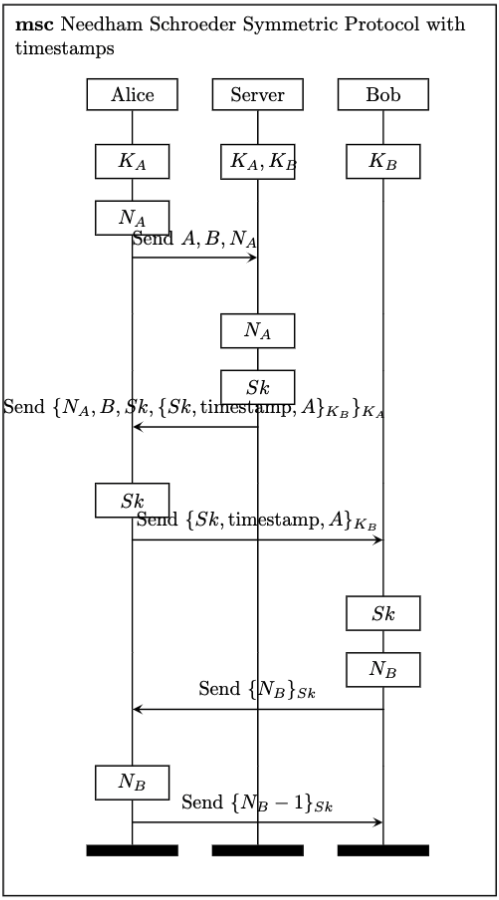
\includegraphics[width=0.45\textwidth]{Figures/NS_fixed.png}
    \label{fig:NS_fixed}
    \caption{Needham-Schroeder protocol with added timestamps}
\end{figure}
%\begin{msc}{Needham Schroeder Symmetric Protocol with timestamps}
    \declinst{alice}{}{Alice}
    \declinst{server}{}{Server}
    \declinst{bob}{}{Bob}
    \action*{ \begin{minipage}{1cm}\centering $K_A$ \end{minipage} }{alice}
    \action*{ \begin{minipage}{1cm}\centering $K_A, K_B$ \end{minipage} }{server}
    \action*{ \begin{minipage}{1cm}\centering $K_B$ \end{minipage} }{bob}
    \nextlevel[2]
    \action*{ \begin{minipage}{1cm}\centering $N_A$ \end{minipage} }{alice}
    \nextlevel[2]
    \mess{Send $A, B, N_A$}{alice}{server}
    \nextlevel[2]
    \action*{ \begin{minipage}{1cm}\centering $N_A$ \end{minipage} }{server}
    \nextlevel[2]
    \action*{ \begin{minipage}{1cm}\centering $Sk$ \end{minipage} }{server}
    \nextlevel[2]
    \mess{Send $\{N_A, B, Sk, \{Sk, \textrm{timestamp}, A\}_{K_B} \}_{K_A}$}{server}{alice}
    \nextlevel[2]
    \action*{ \begin{minipage}{1cm}\centering $Sk$ \end{minipage} }{alice}
    \nextlevel[2]
    \mess{Send $\{Sk, \textrm{timestamp}, A\}_{K_B}$}{alice}{bob}
    \nextlevel[2]
    \action*{ \begin{minipage}{1cm}\centering $Sk$ \end{minipage} }{bob}
    \nextlevel[2]
    \action*{ \begin{minipage}{1cm}\centering $N_B$ \end{minipage} }{bob}
    \nextlevel[2]
    \mess{Send $\{N_B\}_{Sk}$}{bob}{alice}
    \nextlevel[2]
    \action*{ \begin{minipage}{1cm}\centering $N_B$ \end{minipage} }{alice}
    \nextlevel[2]
    \mess{Send $\{N_B-1\}_{Sk}$}{alice}{bob}
\end{msc}

To model this version of the protocol we must change the rules that formalize the intermediate exchanges to include such timestamps:

\begin{lstlisting}[language=Tamarin]
rule Server_answers_request :
    let
        message_to_bob = senc(<~sk, ~timestamp, alice>, kb)
        message_to_alice = senc(<nonce, bob, ~sk, message_to_bob>, ka)
    in
    [
        !Server(alice, ka),
        !Client(alice, ka),
        !Client(bob, kb),
        In(<alice, bob, nonce>),
        Fr(~sk),
        Fr(~timestamp)
    ]
    --[ ServerSendsToAlice(message_to_alice),
        Secret(~sk) ]->
    [
        Out(message_to_alice)
    ]
\end{lstlisting}

\begin{lstlisting}[language=Tamarin]
rule Alice_receives_answer :
    let
        message_to_bob = senc(<sk1, timestamp, alice>, k)
        message_to_alice = senc(<nonce, bob, sk, message_to_bob>, ka)
    in
    [
        !Client(alice, ka),
        !Client(bob, kb),
        AliceQueriesServer(alice, bob, nonce),
        In(message_to_alice)
    ]
    --[ AliceReceivesAnswer(message_to_alice, nonce, message_to_bob, sk, ka),
        AliceSendsToBob(message_to_bob),
        SecretEstablished(alice, bob, sk) ]->
    [
        ExchangeInitiated(alice, bob, sk),
        Out(message_to_bob)
    ]
\end{lstlisting}

\begin{lstlisting}[language=Tamarin]
rule Bob_responds_to_Alice :
    let
        message_from_alice = senc(<sk, timestamp, alice>, kb)
        encrypted_nonce = senc(~nonce, sk)
    in
    [
        In(message_from_alice),
        Fr(~nonce),
        !Client(alice, ka),
        !Client(bob, kb),
        !Server(bob, kb)
    ]
    --[ BobReceivesFromAlice(message_from_alice, sk, kb),
        SecretEstablished(bob, alice, sk, timestamp),
        BobSendsNonce(encrypted_nonce) ]->
    [
        SessionPending(bob, alice, ~nonce, sk),
        Out(encrypted_nonce)
    ]
\end{lstlisting}

We also must introduce a new restriction that models the checking of the timestamp by Bob:

\begin{lstlisting}[language=Tamarin]
restriction CheckingTimestamps :
    "All alice bob sk timestamp #t1 #t2 .
        SecretEstablishedWithTimestamp(bob, alice, sk, timestamp) @ #t1 &
        SecretEstablishedWithTimestamp(bob, alice, sk, timestamp) @ #t2
            ==> #t1 = #t2"
\end{lstlisting}

We can see now that Tamarin when run on the \lstinline|Attack| lemma is not able now to provide any valid trace, thus confirming that this attacks was solved.

\subsubsection{Perfomance metrics}

By running Tamarin on the files that contain the theories formalizing the protocol in the two forms, we will obtain the evaluation of the formulas modeling the security properties. Assuming that we want to analyze the theory of the unfixed Needham-Schroeder protocol contained in \lstinline|./NS.spthy|, we will obtain the following output:

\begin{lstlisting}[language=Terminal]
>>> tamarin-prover NS.spthy

================================================
summary of summaries:

analyzed: NS.spthy

  types (all-traces): verified (45 steps)
  Sanity (exists-trace): verified (15 steps)
  Confidentiality (all-traces): verified (64 steps)
  Attack (exists-trace): verified (18 steps)

================================================
\end{lstlisting}

Similarly, by analyzing the formalization of the fixed protocol contained within file \lstinline|./NS_fixed.spthy|, the tool provides the following result:

\begin{lstlisting}[language=Terminal]
>>> tamarin-prover NS_fixed.spthy

================================================
summary of summaries:

analyzed: NS_fixed.spthy

  types (all-traces): verified (130 steps)
  Sanity (exists-trace): verified (15 steps)
  Confidentiality (all-traces): verified (19 steps)
  Attack (exists-trace): falsified - no trace found (294 steps)

================================================
\end{lstlisting}

In order to gain some insight on the tool's performance, we can measure the time and space resources required by a series of executions of the prover on the single lemmas and calculate some statistics on it. Automating such procedure is pretty straightforward in any modern programming language, and in our case we chose to use Python along to GNU's \lstinline|time| command line utility \cite{GNUtime}:

\begin{table*}[t]
    \centering
    \begin{tabularx}{0.85\textwidth}{@{}lcccccccccc@{}}
        \toprule
        \multicolumn{1}{c}{} & \multicolumn{1}{c}{} & \multicolumn{4}{c}{Duration [ms]} & \multicolumn{4}{c}{Peak RAM usage [kB]}\\
        \cmidrule(rl){3-6} \cmidrule(rl){7-10}
        Lemma & \# of steps & Mean & Max & Min & Deviation & Mean & Max & Min & Deviation \\
        \midrule
        types & 123 & 697 & 770 & 660 & 15.09 & 46697 & 51248 & 44976 & 1295.62\\
        \addlinespace
        Sanity & 15 & 701 & 800 & 670 & 18.20 & 46973 & 50208 & 44016 & 1316.64\\
        \addlinespace
        Confidentiality & 98 & 706 & 770 & 660 & 14.75 & 46957 & 50224 & 43984 & 1357.73\\
        \addlinespace
        Attack & 19 & 745 & 800 & 710 & 16.60 & 46702 & 51232 & 44992 & 1340.96\\
        \bottomrule
        \end{tabularx}
    \caption{Tamarin's performances during the verification of the Needham Schoroeder Symmetric protocol}
    \label{tab:tableNS}
\end{table*}

\begin{table*}[t]
    \centering
    \begin{tabularx}{0.85\textwidth}{@{}lcccccccccc@{}}
        \toprule
        \multicolumn{1}{c}{} & \multicolumn{1}{c}{} & \multicolumn{4}{c}{Duration [ms]} & \multicolumn{4}{c}{Peak RAM usage [kB]}\\
        \cmidrule(rl){3-6} \cmidrule(rl){7-10}
        Lemma & \# of steps & Mean & Max & Min & Deviation & Mean & Max & Min & Deviation \\
        \midrule
        types & 130 & 912 & 1000 & 850 & 37.11 & 61134 & 63504 & 58352 & 875.15\\
        \addlinespace
        Sanity & 15 & 935 & 990 & 870 & 24.51 & 61155 & 62528 & 58288 & 912.24\\
        \addlinespace
        Confidentiality & 19 & 953 & 1040 & 900 & 28.58 & 61132 & 62496 & 59360 & 761.72\\
        \addlinespace
        Attack & 294 & 989 & 1510 & 890 & 86.09 & 61195 & 64528 & 59376 & 786.25\\
        \bottomrule
        \end{tabularx}
    \caption{Tamarin's performances during the verification of the Needham Schoroeder Symmetric protocol after fixing}
    \label{tab:tableNSFixed}
\end{table*}

\begin{lstlisting}[language=Python]
import subprocess, re, json
from statistics import mean, stdev

def runTamarin(filename, lemmaName) :
    command = f'gtime tamarin-prover {filename}.spthy --prove={lemmaName}'
    process = subprocess.run(
        command.split(),
        stdout=subprocess.PIPE,
        stderr=subprocess.PIPE,
        universal_newlines=True)
    res = process.stderr.split('\n')[-3].split()
    time = list(map(
        int,
        res.split('\:|\.', res[2][:-7])))
    milliseconds = (time[0] * 60 * 1000) +
        (time[1] * 1000) +
        (time[2] * 10)
    maxMemory = int(res[-1][:-13])
    return milliseconds, maxMemory

FILES = ['NS', 'NS_fixed']
LEMMAS = [
    'types',
    'Sanity',
    'Confidentiality',
    'Attack']
N_ITERATIONS = 100

out = {}
for file in FILES :
    for lemma in LEMMAS :
        times = []
        mems = []
        for i in range(N_ITERATIONS) :
            res = runTamarin(file, LEMMAS[0])
            times.append(res[0])
            mems.append(res[1])
        out[lemma] = {}
        out[lemma]['maxTime'] = max(times)
        out[lemma]['maxMemory'] = max(mems)
        out[lemma]['minTime'] = min(times)
        out[lemma]['minMemory'] = min(mems)
        out[lemma]['avgTime'] = mean(times)
        out[lemma]['avgMemory'] = mean(mems)
        out[lemma]['stdevTime'] = stdev(times)
        out[lemma]['stdevMemory'] = stdev(mems)
    with open(f'output_{file}.json', 'w') as f:
        json.dump(out, f)
\end{lstlisting}

The script described above measures the resources used to prove each lemma during 100 different iterations. Note that each iteration requires a precomputation-phase overhead, which could be easily amortized by computing all the lemmas in the same execution. The results of our experimentation as described in tables \ref{tab:tableNS} and \ref{tab:tableNSFixed}.

As we can see, with this toy-protocol example, Tamarin is able to prove all the properties in the blink of an eye. Of course, when considering more complex formalizations with additional rules and bigger equational theories involved (such as the \lstinline|diffie-hellman| or the \lstinline|xor| built-ins), the proving process becomes more time-consuming (and often non-terminating). For example, in the reference GitHub repository \cite{github} for this paper it is also possible to find a Tamarin formalization of the X3DH exchange \cite{x3dh} that, despite its brevity, manages to get the prover stuck during the precomputation phase due to the high number of Diffie Hellman exchanges required by the protocol.

\section{Conclusions}\label{sec:conclusions}

In this essay we managed to present the Tamarin prover with a top-down approach: starting from a general introduction to the formal verification background, we introduced the actual tool by quickly explaining its syntax and usage. In order to provide a more concrete point of view on the matter, we also presented the Needham Schroeder Symmetric protocol and formalized its message exchange in Tamarin semantics. Then, we used the tool to prove some of its security properties and showed how it could be subject to a simple replay attack. After showing a potential fix to the problem, we proved that the proposed modification did, in fact, eliminated the attack. Finally, we provided some performance metrics on the tool.

The topic of automated formal verification of protocols is currently an area of active research within the symbolic artificial intelligence field. As computer scientists, this allows us to go through a less cumbersome verification process when checking protocols for correctness, while as users this provides us a better sense of trust with regards to the security features of the application we are using, since their exchanges are more easily formalized and verified against attackers.

%----------------------------------------------------------------------------------------
%	ACKNOWLEDGEMENTS
%----------------------------------------------------------------------------------------

% \phantomsection
% \section*{Acknowledgments} % The \section*{} command stops section numbering
% 
% \addcontentsline{toc}{section}{Acknowledgments} % Adds this section to the table of contents
% 
% So long and thanks for all the fish \cite{Figueredo:2009dg, Smith:2012qr}.

%----------------------------------------------------------------------------------------
%	REFERENCE LIST
%----------------------------------------------------------------------------------------

\phantomsection
\bibliographystyle{alpha}
\bibliography{references.bib}

%----------------------------------------------------------------------------------------

\end{document}